\chapter{Music Data Score}
\thispagestyle{empty}

\label{mds}
{\texttt{2016} -- \texttt{2020}}

\bigskip
\smallskip

\section{Purpose}
\label{purp}

This work allows creating a bridge between data as a musical object or as a traditional score notation, and some algorithmic environment in terms of interpretation, analysis and synthesis such as neural network \textsl{Neuromuse3} (N3) and SuperCollider (SC). Then, this applies basically to a text file in order to be interpreted as a data list -- according to some preliminary conversion -- for the learning process in the N3 context, 
or as a SC array in the context of \href{http://doc.sccode.org/Tutorials/Streams-Patterns-Events1.html}{\textit{Streams, Patterns and Events}} and \href{http://doc.sccode.org/Tutorials/Getting-Started/15-Sequencing-with-Routines-and-Tasks.html}{\textit{Sequencing with Routines and Tasks}}, or as a \href{http://doc.sccode.org/Classes/Score.html}{\textit{Score}} in \href{http://doc.sccode.org/Guides/Non-Realtime-Synthesis.html}{\textit{Non-Realtime Synthesis (NRT)}}.

The aims of this article is then a proposition of formatting what I call a Music Data Score (MDS) from a partition, analysis data and midi file -- using some tools for midi conversion attached to the Common Lisp library M2T (see chapter \textsl{\nameref{m2t}}) --, and a guideline of how to use it in the N3 and SC context.

\section{Writing Music Data Score}

The main idea is to list in time a set of parameters as an event with at least duration \myuline{as the first argument}, and according to a specific encoding as raw data or class number relating to any kind of object. In any case, the number of parameters depend on the initial accuracy, and on the teleological object.

The last line is dedicated to the number of grouping as a number of parameters defining an event. It can be added on the same line -- according to the user needs -- for instance the tempo, the number of duration relative to the tempo, the structure as the number of repetition or according to the order number of the phrases and so.

\subsection{Traditional score}
\label{tradscore}

In this case, we group the data as a musical phrase or by measure or by voices with at least the duration and the pitch. It is possible to add any more information such as the level for instance, or any kind of data describing the event. Note that the number of dimension as to be specified on the last line.

\begin{figure}[!hbt]
	\begin{center}
		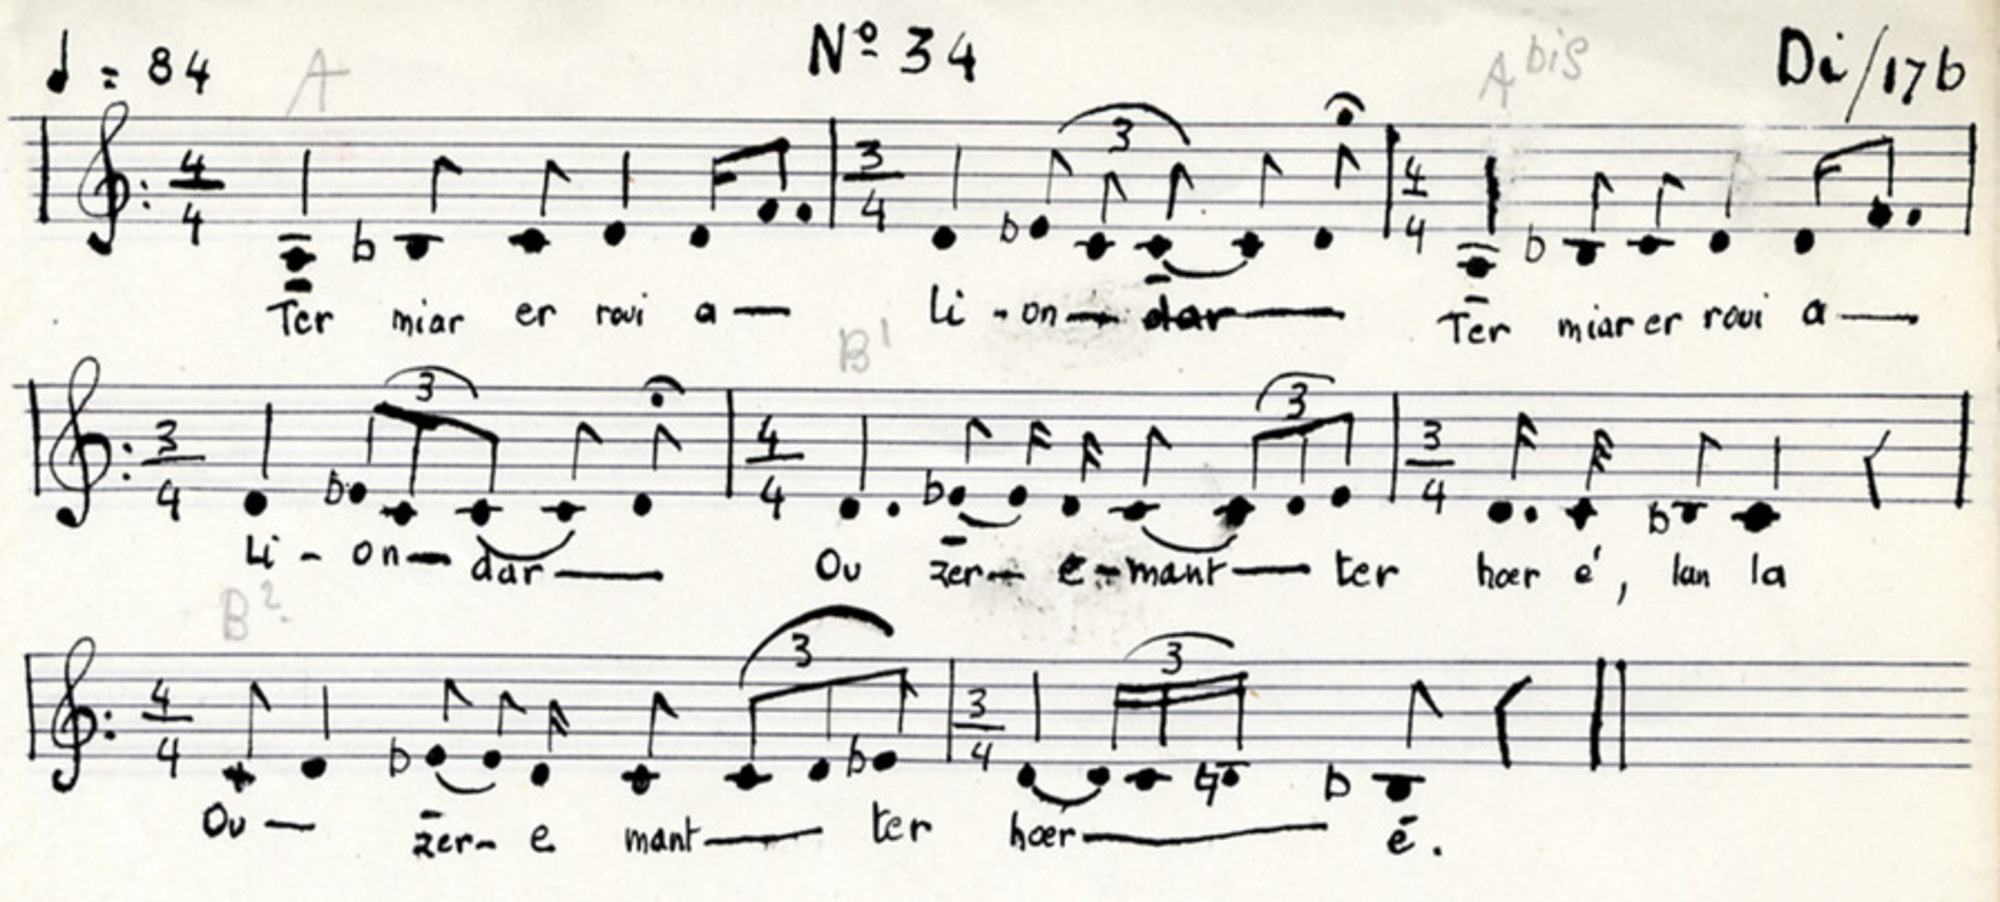
\includegraphics[scale=0.23]{img/2334}
		\caption{Partition of the Breton song \textit{T\`er merh er rou\'e a Liandar} \citep{mbb}.}
		\label{fig:ch34}
	\end{center}
\end{figure}

From a previous work called \texttt{HEX0} (see \fullref{hex0}), the original score in figure \ref{fig:ch34} is encoded according to each bar of the song on 2 lines as follow:

\begin{lstlisting}[language=bash]
24 12 12 24 6 18
57 58 60 62 62 65
24 8 8 20 12+rrand(3,12)
62 63 60 60 62
24 12 12 24 6 18
57 58 60 62 62 65
24 8 8 20 12+rrand(3,12)
62 63 60 60 62
36 18 6 20 8 8
62 63 62 60 62 63
9 3 12 24 24
62 60 58 60 0
12 24 24 6 12 8 8 8
60 62 63 62 60 60 62 63
28 4 4 12 24
62 60 59 58 0
2 84 24 9
\end{lstlisting}

\begin{itemize}
\item The first line represents the durations as integer according to an irreducible minimum value applied for the whole score.
\item The second line represents the midi notes; the zero represents silence; the negative midi note represents a tie to the previous one as absolute value.
\item Some `extra' text can be added depending of the context as for instance in the present case a fermata in the SuperCollider context --  coded \texttt{n+rrand(a,b)} -- which is evaluated between \texttt{n+a} and \texttt{n+b}.
\end{itemize}

 The last line indicates for the first argument the dimension of the events -- with the command line \textsl{enkode} (see chapter \fullref{enk}) this number is 5 -- and optionally the tempo, the number of the irreducible minimum value to fit the whole note of the tempo, and the structure of the piece (can be for instance a number of repetition -- 9 in the example of the Breton song -- for the whole score or a structure such as ABBAC).

\subsection{Analysis data}

The data file has to be ordered in order to list all respective parameters for each event as a row or as a column.

Note that a matrix transposition can be required with the instance method \texttt{flop} in SuperCollider context -- or with the Bash function \textsl{\nameref{trans}} in appendice \fullref{trans}.

\bigskip 

From a sound file, the command line \textsl{enkode} according to an automatic segmentation, generate a list of analysis data by event as duration, $f0$, centroid, loudness and `loudbass'. According to the option, the result is the raw data or a classification by classes (see \fullref{enk:dic}).

\subsection{Reading MDS in SC}
\label{mds2sc}

\begin{lstlisting}[language=Java]
// Read file as array
~score = FileReader.readInterpret("".resolveRelative +/+  
    "dat.score", true, true);
 // -------------------------
~infoLine = ~score.pop;
~grouping = ~infoLine[0];
~score = ~score.clump(~grouping);
// concatenate all `tracks' as musical phrases 
~score=~score.collect({|a| a.flop}).flatten(1).flop;
 // -------------------------
 
// From the cmd line enkode:
// ~score[0] ---> duration
// ~score[1] ---> f0
// ~score[2] ---> centroid
// ~score[3] ---> loudness
// ~score[4] ---> loudbass
\end{lstlisting}

\section{Convert midi file to MDS}
\label{cmftmds}
For any formatted midi file with the extension .mid or .midi there are 2 ways to realize the midi conversion to MDS according to the interpretation it is possible to do either as a sound file or as a data file.

\begin{enumerate}
\item The conversion midi to a sound file formatted as WAV for instance -- in order to compute the MDS as described previously with the command line \textsl{enkode} -- can be done with the command line \texttt{fluidsynth} which requires the SoundFont file \texttt{FluidR3\_GM.sf2} from the package \texttt{fluid-soundfont-gm}.
\begin{lstlisting}[language=bash]
fluidsynth -F outfile.wav /usr/share/sounds/sf2/FluidR3_GM.sf2 infile.mid
\end{lstlisting}
\item The conversion midi to MDS can be done as a raw data -- see \textsl{\nameref{infomidi}} in appendice \fullref{infomidi} -- using some extra tools of the Common Lisp library M2T which is described in the two next sections \textsl{Duration} and \textsl{Score}. Note that this library requires in this case the package MIDI. 

\end{enumerate}

\subsection{Duration}

For each track of the midi file.

\subsubsection{In time}

The duration in time is the difference between the value of the \texttt{Note\_on} and the value of the \texttt{Note\_off} or the same value \texttt{Note\_on} with the level set to zero.

In the case of multi-voices part, there is a bias in terms of fitting the duration between two notes or two chords. If the duration is too long, then it is clipped at the beginning of the next event. Needless to say this bias can be avoid if the score is written with only one voice by track. If the duration stops before the next event and if the remaining duration is significative\footnote{This is another bias about the remaining silence. This last does not have to be under the value of the sixty-fourth note
%, or has to be close to neighboring values.
by default according to the division value of the midi score.}, a silence is set in between. Note that a silence is set to zero as a midi value.

This is done as follow:

\noindent Let $t$ be the position in time of a $chord$ as a group of notes and $d$ the duration.

\noindent Let $A_i$ be the dataset $[ t_i, d_i, chord ]$ at the position $i$.

\noindent Assume that $\delta_i = t_{i+1} - t_i$ and $\Delta_i = \delta_i - d_i$.

\noindent Then,

if $\Delta_i = 0 \rightarrow A_i$

if $\Delta_i > 0 \rightarrow A_i + [ t_i + d_i, \delta_i - d_i, rest ]$

if $\Delta_i < 0 \rightarrow [ t_i, \delta_i, chord ]$

\subsubsection{Out time}

All the durations computed just below are reduced in order to get the minimal value as an integer. This is done by calculating the greatest common divisor using the method of prime factorisations.

\subsection{Score}
\label{score}

In order to illustrate how to manage the midi conversion to the MDS, here are some code snippets in the context of N3 and SC using the score Kj{\o}lhiea from the performances \texttt{K540} (see \fullref{k540}) which was exported as a midi file.

\smallskip

In this case, the scope of the possible division according to the time division of the midi file is set to \texttt{(1 2 4 8)}, that is to say respectively the quarter note, the eighth note, the sixteenth note and the thirty-second note.

\begin{lstlisting}[language=Lisp]
M2T> (setf *scope* '(1 2 4 8))
\end{lstlisting}

\subsubsection{to N3}

In the N3 context, the aim is to format the MDS as an irreducible sonic object in order to be interpreted as an `\textit{infon}', that is to say a clique which can be learned as such. Here, the data has to be ordered according to the network involved, matching each track or voice with its respective SOM (Self organizing Map as a neural network called MLT in N3). 

\smallskip

In this way, the MDS is transposed as a matrix with the relative duration followed by the midi note for each voice of the midi score. 

\begin{lstlisting}[language=Lisp]
M2T> (midi2mds (add-tie (scoring-midi "~/Kjolheia.mid")) 
   :to 'N3)
((2 54 47 62 62) (2 59 62 59 66) (2 59 66 61 66) 
 (2 59 62 54 66) (2 62 64 59 62) (2 59 62 47 67) 
 (1 59 61 64 66) (1 -59 -61 62 -66) (1 59 66 61 67) 
 (1 -59 -66 62 -67) (2 66 47 55 64) (2 59 62 59 67)...
\end{lstlisting}

Note that the function \texttt{add-tie} is applied for each track of the score.


\subsubsection{to SC}

For the performances \texttt{K540}, the midi file Kj{\o}lhiea has been converted to a MDS file as follow:
\begin{lstlisting}[language=Lisp]
M2T> (midi2mds (mix-track (scoring-midi "~/Kjolheia.mid")) 
   :out "~/Kjolheia" :to 'SC)
\end{lstlisting}

Note that the function \texttt{mix-track} allows mixing $n$ tracks or voices to one.
\newpage

The resulting score is formatted as a couple of lines respectively duration and midi note(s) as an array by track as follow:

\begin{lstlisting}[language=bash]
2 2 2 2 2 2 1 1 1 1 2 2 2 2 2 2 2 2 2 2 2 2 2 2 2 2 2 1...
[62,47,54] [66,62,59] [61,66,59] [66,54,62,59] [59,64,6...
2
\end{lstlisting}

\smallskip

Then, we can interpret the MDS in the SuperCollider context according to the section \fullref{mds2sc}. Mind to set a duration factor according to the tempo required.

\smallskip

Thus, the score is interpreted as an array and therefore can be read inside a stream in the Routine or part of Pattern -- using \texttt{Pbind} for instance.
%\newpage¨


\section{Discussion}

This proposition is a satisfying compromise for fixed scores as dataset for `non-real-time synthesis'. Indeed, MDS retains a partition which allows any kind of structural or formal analysis de facto \textit{a posteriori} and algorithmically, on the understanding that does not solve the discrimination issue of the sonic object as an irreducible and signifier axiom. 

\bigskip 

Finally, it is also convenient as a file that can be read in different contexts such as  \textsl{Neuromuse3} or SuperCollider to name but two which have been outlined in this article, and easy to write from traditional score or midi file, even to generate from or as raw data.

\bigskip 

%Concerning the conversion of midi files to MDS, this remains a proposition because, in some context, it will be not enough to reduce some durations as described in the chapter \textsl{Duration} section \textsl{In time}. Also, more information can be selected from the midi file, such as the level and the midi instrument. Another point, for now, each track is computed independently, and this should be able to merge from any track to any other track.

%This will be part of further development if required.


